\chapter[The PAC-Bayesian Theory and the Majority Vote]{The PAC-Bayesian Theory and the Majority Vote}
\label{chap:pac-bayes}
\addchapterlof
\addchapterloe
\addchapterloa

\minitoc

\begin{abstract}
    \looseness=-1
    In this chapter, we introduce, with more details, the PAC-Bayes theory that we outlined in \Cref{chap:intro}.
    This theory allows us to upper-bound the risk of the {\it stochastic} classifier which samples, for each input, a hypothesis to predict the output. 
    Moreover, the risk of the {\it stochastic} classifier can be linked to the {\it majority vote}'s risk;  we remind in this chapter the {\it majority vote classifier} which can be seen as a weighted combination of hypotheses.
    However, when we want to consider only one hypothesis, the {\it disinstegrated} PAC-Bayesian theory becomes more adapted.
    Indeed, it upper-bounds the true risk of a {\it single} hypothesis associated with a high weight.
    Such generalization bounds are recalled as well.
\end{abstract}

\newpage

\section{Introduction}

In this chapter, we details one statistical learning theory that is key in this thesis: the PAC-Bayesian theory.
It is introduced by \citet{ShaweTaylorWilliamson1997,McAllester1998} for which we recall some bounds in \Cref{chap:pac-bayes:sec:pac-bayes}.
This theory assumes that each hypothesis $\h\in\H$ is associated with a (positive) weight $\Q(\h)$ that forms a probability distribution.
Thanks to this assumption, the expected generalization gap is upper-bounded over $\h\sim\Q$. 
The expected generalization gap allows to bound the true risk of the {\it stochastic} classifier; for each input $\x$, the model {\it (i)} samples a hypothesis $\h\sim\Q$ and {\it (ii)} predicts the label with $\h(\x)$.\\

The stochastic classifier is related to a model in which we are particularly interested: the majority vote (see \Cref{chap:pac-bayes:sec:surrogate}).
For instance, majority votes are considered in boosting~\citep{FreundSchapire1996} or bagging~\citep{Breiman1996}.
In this context, a hypothesis is called {\it voter}, and a weight (modeled by the probability distribution $\Q$) is used to define the importance of each voter.
Then, the majority vote is defined as a weighted combination of all the hypotheses from $\H$.\\

A majority vote might bring no significant improvements when the voters are strong (\ie, when their individual risks are small). 
Hence, considering a {\it single} hypothesis associated with a high weight $\Q(\h)$ can be a better option.
Such a classifier is obtained by sampling from the probability distribution $\Q$.
After sampling, generalization guarantees on the classifier can be derived through the {\it disintegrated} PAC-Bayesian bounds introduced independently by \citet{Catoni2007,BlanchardFleuret2007}.
This type of bounds is recalled in \Cref{chap:pac-bayes:sec:disintegrated}.\\

For the sake of completeness, we defer in \Cref{ap:pac-bayes} the proofs.

\section{PAC-Bayesian Majority Votes}

\subsection{Definition}

Given a set of hypotheses $\H$, which is called set of voters in this context, the goal of a majority vote learning algorithm is to find a probability distribution $\Q$ on $\H$.
The distribution $\Q$ defines the weights of the voters, \ie, the importance of each voter in the majority vote.
The majority vote is defined in the following way.

\begin{definition}[Majority Vote]
\looseness=-1
For any hypothesis set $\H$ with voters $\h:\X\to[-1,+1]$, for a distribution $\Q$ on $\H$, the majority vote in the binary classification setting ($\Y=\{-1,+1\}$) is defined as
\begin{align*}
\forall \x\in\X,\quad  \MVQ(\x) \defeq \sign\LP \EE_{\h\sim\Q} \h(\x)\RP.
\end{align*}
In the multi-class setting ($\Y=\{1, 2, \dots, \L\}$), for any hypothesis set $\H$ with voters $\h:\X\to \Y$, the $\Q$-weighted majority vote is defined as
\begin{align*}
\forall \x\in\X,\quad  \MVQ(\x) \defeq \argmax_{\y'\in\Y} \PP_{\h\sim\Q}\LB \h(\x) = \y'\RB = \argmax_{\y'\in\Y}\EE_{\h\sim\Q}\indic\LB \h(\x) = \y'\RB.
\end{align*}
\label{chap:pac-bayes:majority-vote}
\end{definition}

In the binary setting, the majority vote predicts as label the sign associated with the $\Q$-weighted average of the voters' outputs.
In the multi-class setting, the majority vote predicts the label $\y'\in\Y$ with the highest associated score $\PP_{\h\sim\Q}\LB \h(\x) = \y'\RB$.
When the hypothesis set $\H$ is composed of voters $\h:\X\to \{-1,+1\}$ in the binary setting, the majority vote for the multi-class setting can be seen as a generalization.
Indeed, we have $\sign\LP \EE_{\h\sim\Q}\h(\x)\RP=+1$ if $\PP_{\h\sim\Q}\LB \h(\x) = +1\RB \ge \PP_{\h\sim\Q}\LB \h(\x) = -1\RB$ and $\sign\LP \EE_{\h\sim\Q}\h(\x)\RP=-1$ otherwise.\\

While this definition of the majority vote classifier might appear a bit restrictive, it encompasses multiple widespread classifiers.
For example, the Support Vector Machine~\citep{CortesVapnik1995} can be implicitly expressed as a majority vote where each voter depends on one example \citep{GraepelHerbrichShaweTaylor2005}.
The well-known $k$-Nearest Neighbors~\citep{CoverHart1967} is a majority vote~\citep{BelletHabrardMorvantSebban2014}.
Additionally, when the voters depend on the whole learning sample $\S$, neural networks can be seen as a majority vote~\citep{KawaguchiPackKaelblingBengio2017, ViallardGermainHabrardMorvant2019}.\\

There are many approaches to learn a majority vote classifier based on ensemble methods.
For example, the bagging~\citep{Breiman1996} method splits the learning sample and learns one voter with each subset.
Then, the majority vote classifier averages the decision of the voters to take the final decision; random forest~\citep{Breiman2001} is, for instance, a particular bagging algorithm for decision trees.
Moreover, the weights $\Q$ can be learned greedily: this is the purpose of boosting algorithms such as Adaboost~\citep{FreundSchapire1996}.
This algorithm has been improved in various directions, \eg, for the multi-class setting~\citep{SchapireSinger1998,SchapireSinger1999,SchapireSinger2000,ZhuZouRossetHastie2009} or the ranking setting with RankBoost~\citep{FreundIyerSchapireSinger1998,FreundIyerSchapireSinger2003}.
Boosting algorithms have also been generalized for differentiable loss functions in a method called gradient boosting~\citep{Friedman2001}.\\

Given a distribution $\Dp$ on $\X\times\Y$ (that encompasses the distributions $\D$ and $\dS$), the learner wants to learn $\MVQ$ that commits as few errors as possible on $\D$.
To reduce the number of errors of the majority vote $\MVQ$ on $\Dp$, the learner aims to minimize the risk $\Risk_{\Dp}(\MVQ)$ under the 01-loss in the following definition.

\begin{definition}[Risk of the Majority Vote]
For any distribution $\Dp$ on $\X\times\Y$, for any hypothesis set $\H$, for any distribution $\Q$ on $\H$, the risk of the majority vote is defined as 
\begin{align*}
\Risk_{\Dp}(\MVQ) \defeq \EE_{(\x, \y)\sim\Dp} \indic\LB \MVQ(\xbf) \ne \y\RB =\PP_{(\x,\y)\sim\Dp}\LB \MVQ(\x) \ne \y \RB.
\end{align*}
\label{chap:pac-bayes:def:mv-risk}
\end{definition}

Specifically, when $\Dp=\D$, the risk $\Risk_{\Dp}(\MVQ){=}\Risk_{\D}(\MVQ)$ is the true risk of the majority vote and when $\Dp=\dS$ the risk $\Risk_{\Dp}(\MVQ){=}\Risk_{\dS}(\MVQ)$ is the empirical risk of the majority vote.
In order to gain insight into the majority vote's decision, the margin captures how much the classifier makes errors.
Indeed, the majority vote's risk can be expressed in terms of the margin defined in the following way. 

\begin{definition}[Margin of the Majority Vote]
For any hypothesis set $\H$, for any distribution $\Q$ on $\H$, the margin of the majority vote is defined as
\begin{align*}
    \MaQ(\x,\y) \defeq \PP_{\h\sim\Q}\LB \h(\x)=\y \RB - \max_{\y'\in\Y, \y'\ne\y}\PP_{\h\sim\Q}\LB \h(\x)=\y' \RB.
\end{align*}
\end{definition}


\begin{figure}[t]
    \centering
    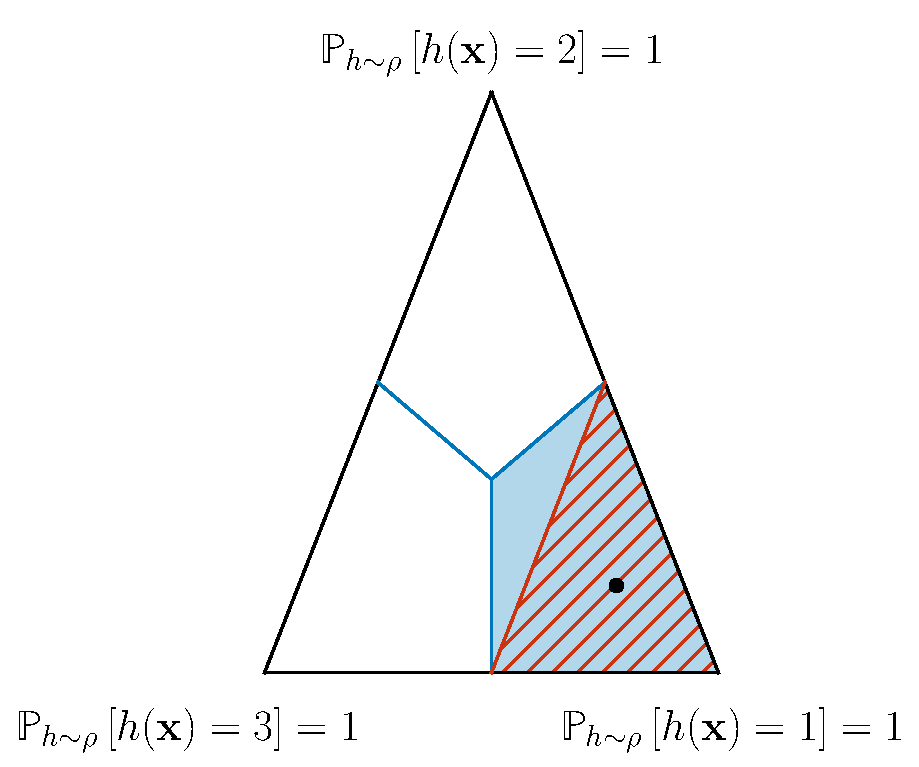
\includegraphics[width=0.5\textwidth]{chapter_2/figures/margin.pdf}
    \caption[Illustration of the Margin of the Majority Vote]{%
    Illustration of the majority vote's margin in the multi-class setting with 3 classes, \ie, $\Y=\{1, 2, 3\}$.
    The triangle represents the ternary plot of the three scores where each triangle's vertex is the three possible maximum scores with $\PP_{\h\sim\Q}\LB \h(\x)=i \RB=1$ for all $i\in\Y$.
    The black dot represents the prediction of an example $(\x, \y)\in\X\times\Y$ by the majority vote: the scores are $\PP_{\h\sim\Q}\LB \h(\x)=1 \RB=0.7$ and $\PP_{\h\sim\Q}\LB \h(\x)=2 \RB=\PP_{\h\sim\Q}\LB \h(\x)=3 \RB=0.15$.
    The blue area is where the majority vote predicts the label $\y$ for the input $\x$ and where the margin $\MaQ(\x,\y)$ is positive.
    Whereas the red area represents the predictions where $\PP_{\h\sim\Q}\LB \h(\x)=1 \RB\ge\frac{1}{2}$ (\ie, where the $\frac{1}{2}$-margin $\OmMaQ(\x,\y)$ is positive).
    }
    \label{chap:pac-bayes:fig:margin}
\end{figure}

The margin is positive if the score $\PP_{\h\sim\Q}\LB \h(\x)=\y \RB$ is higher than the score associated with the other labels $\y'\ne \y$ and is negative otherwise.
It captures if an example $(\x,\y)\sim\Dp$ is misclassified.
Indeed, thanks to the margin, the majority vote's risk $\Risk_{\Dp}(\MVQ)$ can be rewritten as follows:
\begin{align*}
\Risk_{\Dp}(\MVQ) &= \PP_{(\x,\y)\sim\Dp}\LB \PP_{\h\sim\Q}\LB \h(\x)=\y \RB \le \max_{\y'\in\Y, \y'\ne\y}\PP_{\h\sim\Q}\LB \h(\x)=\y' \RB \RB\\
&= \PP_{(\x,\y)\sim\Dp}\LB \MaQ(\x, \y) \le 0\RB.
\end{align*}

Hence, the risk is the probability that one of the scores is higher than the one of the correct label.
Unfortunately, deriving a learning algorithm to optimize the margin can be challenging since it is non-convex \wrt the posterior $\Q$ because of the $\max$.
To overcome this issue, \citet{LavioletteMorvantRalaivolaRoy2017} propose to consider a convex lower bound of the true margin called $\frac{1}{2}$-margin\footnote{We multiply the $\frac{1}{2}$-margin of \citet{LavioletteMorvantRalaivolaRoy2017} by two.}.

\begin{definition}[$\frac{1}{2}$-Margin of the Majority Vote]
For any hypothesis set $\H$, for any distribution $\Q$ on $\H$, the $\frac{1}{2}$-margin is defined as
\begin{align*}
    \OmMaQ(\x,\y) = 2\LB\PP_{\h\sim\Q}\LB \h(\x)=\y \RB - \frac{1}{2}\RB.
\end{align*}
\label{chap:pac-bayes:def:1/2-margin}
\end{definition}

When the score $\PP_{\h\sim\Q}\LB \h(\x)=\y \RB$ exceeds $\frac{1}{2}$, the majority vote surely classifies correctly the example $(\x, \y)\sim\Dp$.
Hence, the idea of this margin is to compute the difference between the score and $\frac{1}{2}$: when the margin is positive, the example is correctly classified.
We illustrate the difference between the two margins in \Cref{chap:pac-bayes:fig:margin}.
In binary classification, the $\frac{1}{2}$-margin boils down to $\OmMaQ(\x,\y) = \y\EE_{\h\sim\Q}\h(\x) = \EE_{\h\sim\Q}\Mah(\x,\y)$ (which is the margin introduced in \Cref{chap:intro:sec:loss-risk}).
From \Cref{chap:pac-bayes:def:1/2-margin}, we can deduce the following upper bound on the majority vote's risk, \ie, we have  
\begin{align*}
    \Risk_{\Dp}(\MVQ) &\le \PP_{(\x,\y)\sim\Dp}\LB \PP_{\h\sim\Q}\LB \h(\x)=\y \RB \le \frac{1}{2}\RB = \PP_{(\x,\y)\sim\Dp}\LB \OmMaQ(\x,\y) \le 0\RB.
\end{align*}

In general, the majority vote's risk $\Risk_{\Dp}(\MVQ)$ is not practical in learning algorithms because the gradient is zero (see \Cref{chap:intro:sec:loss-risk}).
Hence, in the next section, we recall different upper bounds on the majority vote's risk considered as surrogate losses.

\subsection{Upper Bounds on the Majority Vote's Risk}
\label{chap:pac-bayes:sec:surrogate}

We recall three surrogates on the majority vote's risk introduced in the literature, namely, the Gibbs Risk~\citep{LangfordShaweTaylor2002,McAllester2003}, the joint error~\citep{LacasseLavioletteMarchandGermainUsunier2006,GermainLacasseLavioletteMarchandRoy2015,MasegosaLorenzenIgelSeldin2020}, and the C-Bound~\citep{Breiman2001,LacasseLavioletteMarchandGermainUsunier2006,RoyLavioletteMarchand2011}.
We make use of these surrogate in \Cref{part:contrib-pac-bayes} to derive self-bounding learning algorithms.\footnote{A self-bounding algorithm, coined by \citet{Freund1998}, is a learning algorithm that comes with a generalization guarantee.}
More precisely, in \Cref{chap:mv-robustness}, we leverage the Gibbs risk for the adversarially robust setting and, in \Cref{chap:mv}, we learn majority vote classifiers through the C-Bound.

\subsubsection{The Gibbs Risk}

The first surrogate on the risk $\Risk_{\Dp}(\MVQ)$ introduced in the PAC-Bayesian literature is the {\it Gibbs risk} \citep{LangfordShaweTaylor2002,McAllester2003}.
This risk gives the average performance of individual voters in the majority vote. 
It is defined in the following way. 

\begin{definition}[Gibbs Risk]\label{chap:pac-bayes:def:gibbs} For any distribution $\Dp$ on $\X\times\Y$, for any hypothesis set $\H$, for any distribution $\Q$ on $\H$, the {\it Gibbs risk} is defined as
\begin{align*}
r_{\Dp}(\Q) \defeq \EE_{(\x,\y)\sim\Dp}   \EE_{\h\sim \Q} \indic\LB\h(\x) \ne \y\RB = \PP_{(\x,\y)\sim\Dp, \h\sim\Q}\LB \h(\x) \ne \y \RB.
\end{align*}
\end{definition}

Put into words, the Gibbs risk is the $\Q$-weighted average of the voters' risk.
Moreover, we can write the Gibbs Risk with respect to the $\frac{1}{2}$-margin. Indeed, we have 
\begin{align}
    r_{\Dp}(\Q) = \frac{1}{2}\LB 1-\EE_{(\x,\y)\sim\Dp}\OmMaQ(\x,\y)\RB.\label{chap:pac-bayes:eq:gibbs-margin}
\end{align}

\citet{LangfordShaweTaylor2002} show that the majority vote's risk is upper-bounded by twice the Gibbs risk.
The inequality is recalled in the following theorem. 

\begin{restatable}[Risk Upper Bound Based on the Gibbs Risk]{theorem}{theoremgibbs}\label{chap:pac-bayes:theorem:2gibbs} 
\looseness=-1
For any distribution $\Dp$ on $\X\times\Y$, for any hypothesis set $\H$, for any distribution $\Q$ on $\H$, we have
\begin{align}
\Risk_{\Dp}(\MVQ) \leq 2\, r_{\Dp}(\Q).
\label{chap:pac-bayes:eq:2gibbs}
\end{align}
\end{restatable}
\begin{noaddcontents}\begin{proof}
Deferred to~\Cref{ap:pac-bayes:sec:proof-2gibbs}.
\end{proof}\end{noaddcontents}

However, in ensemble methods where one wants to combine voters efficiently, the Gibbs risk appears to be an imprecise surrogate since the combination of voters might compensate for individual errors.
Hence, other surrogates need to be taken into account.

\subsubsection{Joint Error}

The joint error, introduced by \citet{LacasseLavioletteMarchandGermainUsunier2006}, takes better the voters' correlation into account; this quantity is defined in the following way.

\begin{definition}[Joint Error]\label{chap:pac-bayes:def:joint} For any distribution $\Dp$ on $\X\times\Y$, for any hypothesis set $\H$, for any distribution $\Q$ on $\H$, the {\it joint error} is defined as
\begin{align*}
    e_{\Dp}(\Q) &\defeq \EE_{(\x,\y)\sim\Dp} \EE_{\h\sim\Q}\EE_{\h'\sim\Q}
     \indic\LB\h(\x) \ne \y\big]\indic\big[\h'(\x) \ne \y\RB\\
    &= \PP_{(\x,\y)\sim\Dp, \h\sim\Q, \h'\sim\Q}\LB\h(\x) \ne \y, \h'(\x) \ne \y\RB.
\end{align*}
\end{definition}

Similarly to \Cref{chap:pac-bayes:eq:gibbs-margin} for the Gibbs risk, we can reinterpret this surrogate with the $\frac{1}{2}$-margin.
Indeed, from \citet{GermainLacasseLavioletteMarchandRoy2015}, we have 
\begin{align}
    e_{\Dp}(\Q) &= \EE_{(\x,\y)\sim\Dp}\LP \PP_{\h\sim\Q}\LB \h(\x)\ne\y\RB\RP^2\nonumber\\
    &= \EE_{(\x,\y)\sim\Dp}\LP\frac{1}{2}\LB1-\OmMaQ(\x,\y)\RB\RP^2\nonumber\\
    &= \frac{1}{4}\LP 1-2\EE_{\h\sim\Q}\OmMaQ(\x,\y) + \EE_{\h\sim\Q}\OmMaQ(\x,\y)^2\RP.\label{chap:pac-bayes:eq:joint-margin} 
\end{align}

Recently, \citet{MasegosaLorenzenIgelSeldin2020} proposed to deal directly with the joint error to bound the majority vote's risk; Their bound is presented in the following theorem.

\begin{restatable}[Risk Upper Bound Based on the Joint Error]{theorem}{theoremjoint}\label{chap:pac-bayes:theorem:4joint}
\looseness=-1
For any distribution $\Dp$ on $\X\times\Y$, for any hypothesis set $\H$, for any distribution $\Q$ on $\H$, we have
\begin{align}
    \Risk_{\Dp}(\MVQ) \le 4e_{\Dp}(\Q). 
    \label{chap:pac-bayes:eq:4joint}
\end{align}
\end{restatable}
\begin{noaddcontents}\begin{proof}
Deferred to~\Cref{ap:pac-bayes:sec:proof-4joint}.
\end{proof}\end{noaddcontents}

\looseness=-1
This inequality captures the fact that the voters need to be sufficiently diverse and commit errors on different points.
However, when the joint error $e_{\Dp}(\Q)$ exceeds~$\frac14$, the bound exceeds $1$ and is uninformative.
In some cases, these two upper bounds appear to be less tight than another one: the C-Bound~\citep{Breiman2001,LacasseLavioletteMarchandGermainUsunier2006}. 

\subsubsection{The C-Bound}

The C-Bound\footnote{The term ``C-Bound'' was introduced in the PAC-Bayesian literature by \citep{LacasseLavioletteMarchandGermainUsunier2006}.} \citep{Breiman2001,LacasseLavioletteMarchandGermainUsunier2006} is another surrogate (and upper bound) of the majority vote's risk.
It is derived from the \textsc{Chebyshev}-\textsc{Cantelli} Inequality (see \Cref{ap:tools:theorem:cantelli}).
It depends on the {\it Gibbs risk}, the {\it joint error}, and the {\it disagreement}.
This latter is defined in the following way.

\begin{definition}[Disagreement]\label{chap:pac-bayes:def:disagreement} For any distribution $\Dp$ on $\X\times\Y$, for any hypothesis set $\H$, for any distribution $\Q$ on $\H$, the {\it disagreement} is defined as
\begin{align*}
    d_{\Dp}(\Q) &\defeq 2\EE_{(\x,\y)\sim\Dp}\EE_{\h\sim\Q}\EE_{\h'\sim\Q}\indic\LB \h(\x)\ne \y\RB\indic\LB \h'(\x)=\y\RB\\
    &= 2\PP_{(\x,\y)\sim\Dp, \h\sim\Q, \h'\sim\Q}\LB \h(\x)\ne \y, \h'(\x)=\y\RB.
\end{align*}
\end{definition}

The higher the disagreement, the more the voters do not perform the same prediction for a given $(\x,\y)\sim\Dp$.
Similarly to the Gibbs risk and the joint error, we can express the disagreement with the margin.
Indeed, we have
\begin{align}
    d_{\Dp}(\Q) = \frac{1}{2}\LB 1 - \EE_{(\x,\y)\sim\Dp}\OmMaQ(\x,\y)^2\RB.\label{chap:pac-bayes:eq:disagreement-margin}
\end{align}

Interestingly, by developing \Cref{chap:pac-bayes:eq:joint-margin}, we can relate the Gibbs risk and the joint error to the disagreement with
\begin{align}
    d_{\Dp}(\Q) = 2\LB r_{\Dp}(\Q) - e_{\Dp}(\Q)\RB.\label{chap:pac-bayes:eq:disagreement-risk-joint}
\end{align}
This inequality tells us two facts: {\it (i)} the lower the Gibbs risk, the lower the disagreement, and {\it (ii)} the disagreement increases as the joint error decreases.
The expression of the disagreement in binary classification can be simplified (with voters $\h:\X\to \{-1, +1\}$).
Indeed, given an example $(\x, \y)\sim\Dp$ with $\y\in\{-1, +1\}$, we have
\begin{align*}
    \PP_{\h\sim\Q, \h'\sim\Q}\LB \h(\x)\ne\h'(\x)\RB &= \PP_{\h\sim\Q, \h'\sim\Q}\LB \h(\x)=\y, \h'(\x)\ne\y \RB + \PP_{\h\sim\Q, \h'\sim\Q}\LB \h(\x)\ne\y, \h'(\x){=}\y \RB\\
    &= 2\PP_{\h\sim\Q, \h'\sim\Q}\LB \h(\x)\ne \y, \h'(\x)=\y\RB,
\end{align*}
which gives $d_{\Dp}(\Q)=\PP_{(\x,\y)\sim\Dp, \h\sim\Q, \h'\sim\Q}\LB \h(\x)\ne\h'(\x)\RB$.

Thanks to this quantity, we are now able to recall the C-Bound.
Note that it was first introduced by \citet{LacasseLavioletteMarchandGermainUsunier2006} for the PAC-Bayesian majority vote in binary classification.
The generalization to the multi-class setting has been introduced by \citet[Theorem~2 and Corollary~1]{LavioletteMorvantRalaivolaRoy2017}; we recall the C-Bound in the following theorem.

\begin{restatable}[The C-Bound]{theorem}{theoremgeneralcbound}\label{chap:pac-bayes:theorem:cbound}
For any distribution $\Dp$ on $\X\times\Y$, for any hypothesis set $\H$, for any distribution $\Q$ on $\H$, if 
\begin{align*}
\EE_{(\x,\y)\sim\Dp}\OmMaQ(\x,\y) > 0 \iff r_{\Dp}(\Q)<\tfrac{1}{2}\iff2e_{\Dp}(\Q)+d_{\Dp}(\Q)<1,
\end{align*}
we have
\begin{align}
\Risk_{\Dp}(\MVQ) &\le 1-\frac{\LP\EE_{(\x,\y)\sim\Dp}\LB \OmMaQ(\x,\y)\RB\RP^2}{\EE_{(\x,\y)\sim\Dp}\LP \OmMaQ(\x,\y)\RP^2}\label{chap:pac-bayes:eq:multi-class-cbound}\\
&= 1-\frac{\LP1-2r_{\Dp}(\Q)\RP^2}{1-2d_{\Dp}(\Q)}\label{chap:pac-bayes:eq:cbound-r-d}\\
    &= 1-\frac{\big(1-\LB2e_{\Dp}(\Q)+d_{\Dp}(\Q)\RB\big)^2}{1-2d_{\Dp}(\Q)}\label{chap:pac-bayes:eq:cbound-e-d} \\ 
    &= \CBound_{\Dp}(\Q).\nonumber
\end{align}
\end{restatable}
\begin{noaddcontents}\begin{proof}
Deferred to~\Cref{ap:pac-bayes:sec:proof-cbound}.
\end{proof}\end{noaddcontents}

This surrogate is expressed as a trade-off between the first and the second statistical moment of the $\frac{1}{2}$-margin $\OmMaQ(\x,\y)$ (\Cref{chap:pac-bayes:eq:multi-class-cbound}).
Based on \Cref{chap:pac-bayes:eq:gibbs-margin,chap:pac-bayes:eq:disagreement-margin}, the trade-off can be expressed through the the disagreement and the Gibbs risk (see \Cref{chap:pac-bayes:eq:cbound-r-d}).
Moreover, from \Cref{chap:pac-bayes:eq:disagreement-risk-joint}, we can also see the C-Bound as a trade-off between the joint error and the disagreement in \Cref{chap:pac-bayes:eq:cbound-e-d}.\\

The three surrogates of \Cref{chap:pac-bayes:theorem:2gibbs,chap:pac-bayes:theorem:4joint,chap:pac-bayes:theorem:cbound} can be easily compared.
For instance, when $r_{\Dp}(\Q) \leq d_{\Dp}(\Q)$, the C-Bound $\CBound_{\Dp}(\Q)$ (\Cref{chap:pac-bayes:eq:multi-class-cbound}) is tighter than $2r_{\Dp}(\Q)$ (\Cref{chap:pac-bayes:eq:2gibbs}) and $4e_{\Dp}(\Q)$ (\Cref{chap:pac-bayes:eq:4joint}).
Hence, when the disagreement increases, the C-Bound appears to be a good trade-off between the Gibbs risk and the disagreement.
More precisely, the main interest of the C-bound compared to \Cref{chap:pac-bayes:eq:4joint} is that when $e_{\Dp}(\Q)$ is close to $\tfrac{1}{4}$, the C-Bound can be close to $0$ depending on the value of the disagreement $d_{\Dp}(\Q)$: the C-bound is then more precise.
Moreover, it is important to notice that the C-Bound is tighter than $4e_{\Dp}(\Q)$ for all cases.
We summarize the relationships between the different surrogates in the next theorem and illustrate it in \Cref{chap:pac-bayes:fig:cbound}; this relation is notably given by \citet{GermainLacasseLavioletteMarchandRoy2015} and \citet{MasegosaLorenzenIgelSeldin2020}.

\begin{restatable}[Relationship between \Cref{chap:pac-bayes:theorem:2gibbs,chap:pac-bayes:theorem:4joint,chap:pac-bayes:theorem:cbound}]{theorem}{theoremrelationship}\label{chap:pac-bayes:theorem:relationship}
 For any distribution $\D$ on $\X\times\Y$, for any voters set $\H$, for any distribution $\Q$ on $\H$, if $r_{\Dp}(\Q) < \tfrac{1}{2}$ (\ie, $\EE_{(\x,\y)\sim\Dp}\OmMaQ(\x,\y) > 0$), we have
\begin{center}
\begin{enumerate}[\it (i)]
    \item $\Risk_{\Dp}(\MVQ) \le C_{\Dp}(\Q) \le 4e_{\Dp}(\Q) \le 2r_{\Dp}(\Q)$, if  $r_{\Dp}(\Q) \le d_{\Dp}(\Q)$,
    \item $\Risk_{\Dp}(\MVQ) \le 2r_{\Dp}(\Q) \le C_{\Dp}(\Q) \le 4e_{\Dp}(\Q)$,\quad otherwise.
\end{enumerate}
\end{center}
\end{restatable}
\begin{noaddcontents}\begin{proof}
Deferred to~\Cref{ap:pac-bayes:sec:proof-relationship}.
\end{proof}\end{noaddcontents}

\begin{figure}
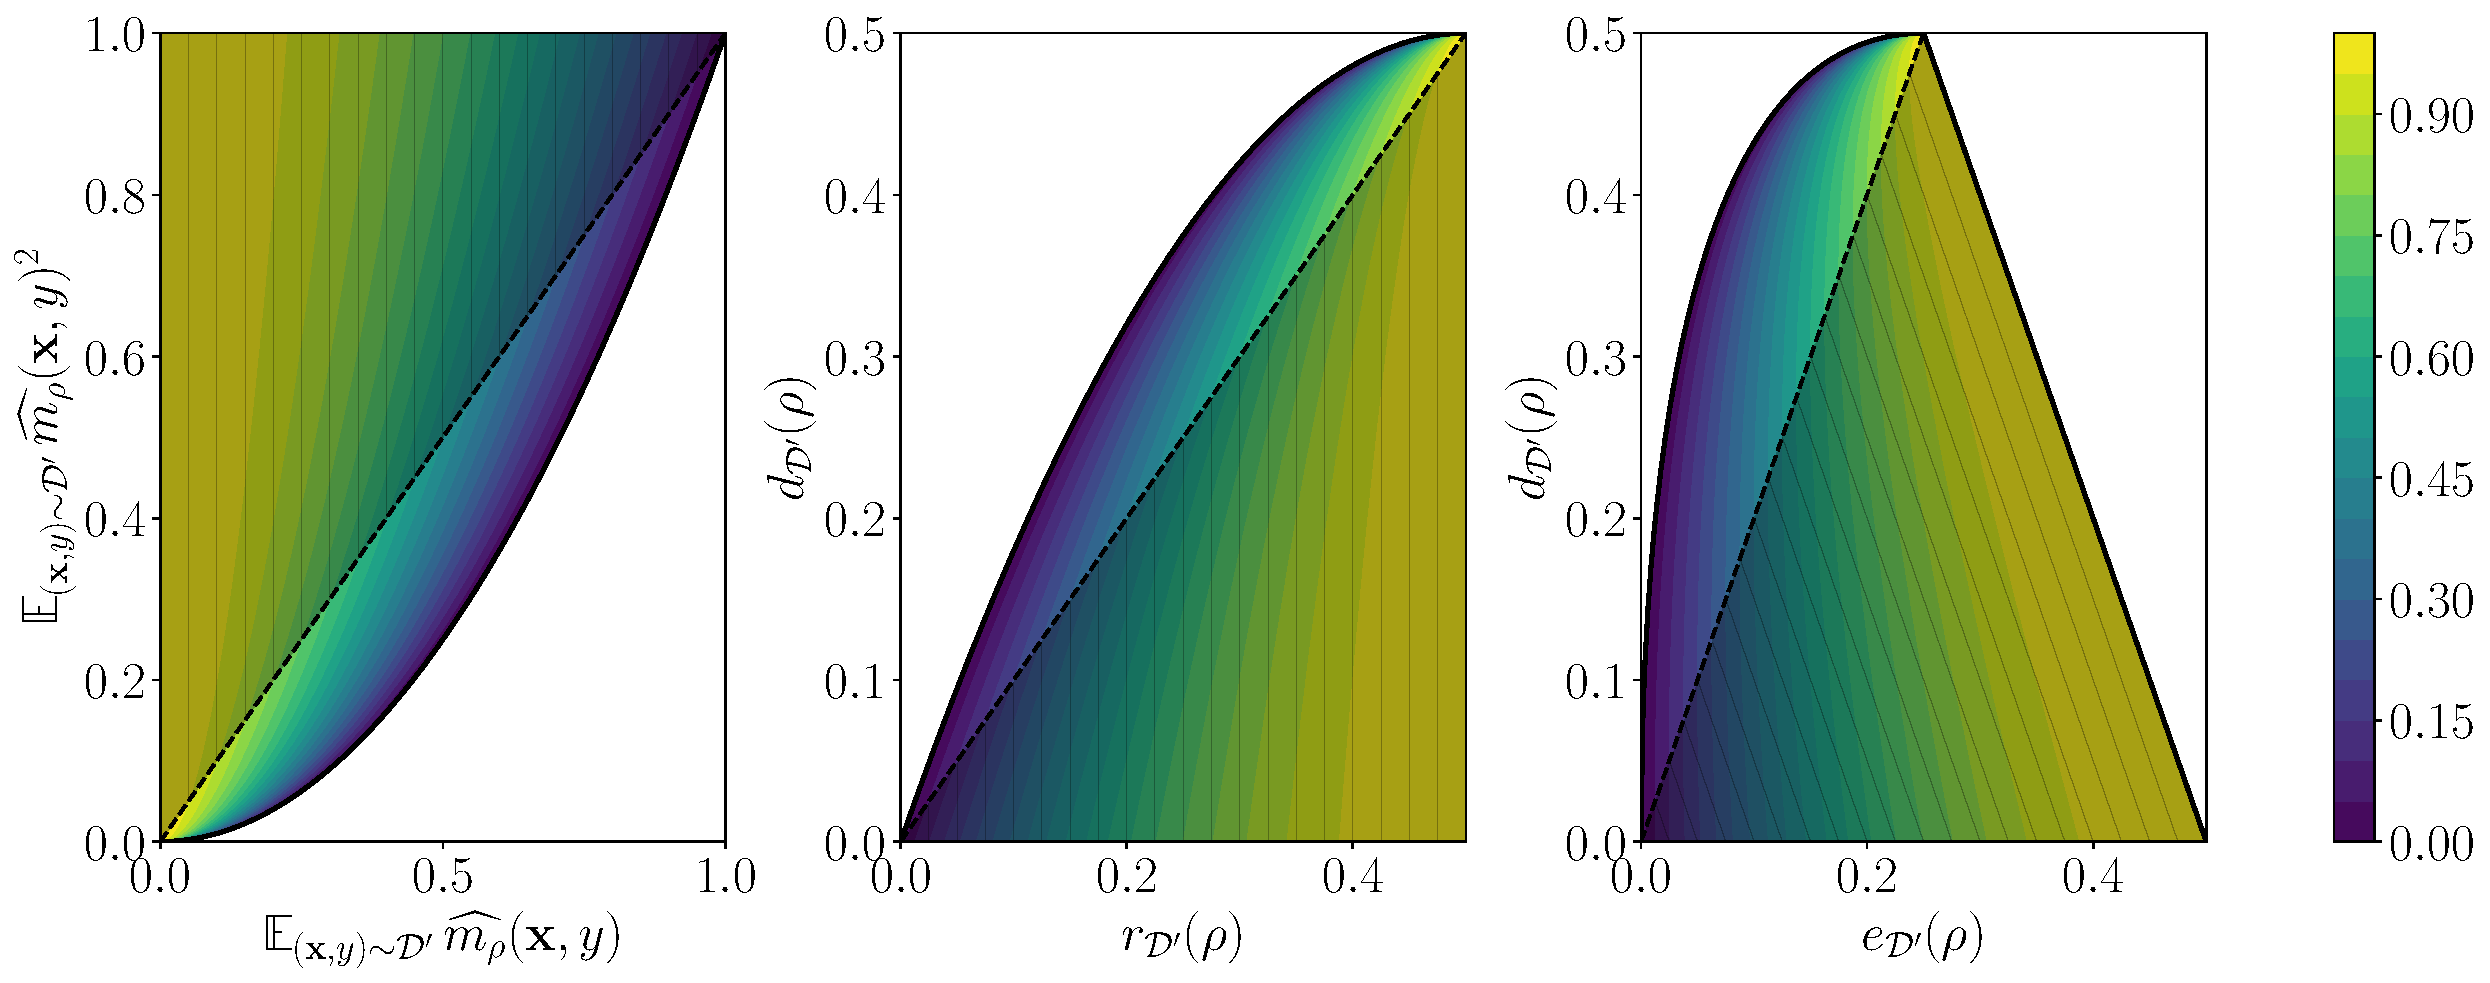
\includegraphics[width=1.0\textwidth]{chapter_2/figures/cbound.pdf}
\caption[Plots that Summarize the Relationship Between the Surrogates]{
Plots (from left to right) of the different C-Bounds in \Cref{chap:pac-bayes:eq:multi-class-cbound,chap:pac-bayes:eq:cbound-r-d,chap:pac-bayes:eq:cbound-e-d}.
For each plot, the darker area represents the cases where $2r_{\Dp}(\Q)$ is tighter than the C-Bound $\CBound_{\Dp}(\Q)$.
The  dashed line represents the cases where $4e_{\Dp}(\Q)$ matches the C-Bound $\CBound_{\Dp}(\Q)$.
}
\label{chap:pac-bayes:fig:cbound}
\end{figure}



Since the distribution $\D$ is unknown, the true risk of the majority vote $\Risk_{\D}(\MVQ)$ is not computable.
Hence, one can minimize the empirical risk of the majority vote $\Risk_{\dS}(\MVQ)$ through the Empirical Risk Minimization approach (see \Cref{chap:intro:algo:erm}).
However, this minimization does not necessarily lead to a low true risk $\Risk_{\D}(\MVQ)$ since overfitting can occur (see \Cref{chap:intro:sec:selection}).
To tackle this issue, one solution is to deal with the minimization of a generalization bound to get a self-bounding algorithm~\citep{Freund1998}, \ie, the  minimization of the risk with generalization guarantees.
We will see in the next section PAC-Bayesian generalization bounds that further allow us to upper-bound the true risk $\Risk_{\D}(\MVQ)$ in \Cref{part:contrib-pac-bayes}.

\section{PAC-Bayesian Bounds}
\label{chap:pac-bayes:sec:pac-bayes}

The PAC-Bayesian theory\footnote{See \citep{Guedj2019,Alquier2021} for recent on the PAC-Bayesian theory.}, introduced by \citet{ShaweTaylorWilliamson1997} and \citet{McAllester1999}, aims to provide PAC generalization bounds for Bayesian-like algorithms.
Such Bayesian algorithms assume a probability distribution defined {\it apriori} on the hypothesis set $\H$, and thanks to Bayes' theorem, obtain an {\it a posteriori} probability distribution on $\H$ thanks to the learning sample; see \citet{Bishop2007} for more details on this Bayesian inference procedure.
Contrary to the classical Bayesian inference where the {\it posterior} distribution is proportional to the product of the {\it prior} distribution and the likelihood of the data, in PAC-Bayesian theory, an arbitrary {\it prior} distribution can be considered.
Actually, the term ``Bayesian'' in the PAC-Bayesian theory comes from the fact that we usually upper-bound the {\it expected} generalization gap $\LN \EE_{\h\sim\AQ}\RiskLoss_{\D}(\h)-\EE_{\h\sim\AQ}\RiskLoss_{\dS}(\h)\RN$ where $\h\in\H$ is sampled from a data-dependent distribution $\AQ$ called {\it posterior}.
This theory has been extended to various settings such as transductive learning~\citep{DerbekoElYanivMeir2004, BeginGermainLavioletteRoy2014}, regression~\citep{GermainBachLacosteLacosteJulien2016, ShalaevaEsfahaniGermainPetreczky2020}, structured prediction~\citep{LavioletteMorvantRalaivolaRoy2017}, domain adaptation~\citep{GermainHabrardLavioletteMorvant2020}, or randomized learning~\citep{London2017}.\\

In order to define a PAC-Bayesian bound more formally, we denote by $\AQ$ (or $\Q$) the {\it posterior} distribution on $\H$ and $\P$ the {\it prior} distribution.
Each probability distribution $\Q$ is defined through its probability density function $\h \mapsto \Q(\h)$ with respect to a reference measure\footnote{For instance, if $\H=\Rbb^{d}$, then the reference measure is the Lebesgue one.} on $\H$; we denote by $\M(\H)$ the set of probability density function on $\H$.
Hence, the distribution $\AQ\in\M(\H)$ is the Radon–Nikodym derivative of a probability measure \wrt the reference measure.
We also denote by $\M^{*}(\H)\subseteq\M(\H)$ the set of strictly positive probability densities on $\H$.
Moreover, for convenience, we assume that the support of the posterior $\AQ$ is in the support of $\P$, \ie, if $\P(\h)=0$ then $\AQ(\h)=0$ (the absolute continuity); hence $\P\in\M^{*}(\H)$.\\

\looseness=-1
With the setting in place, we can now define the general form of a PAC-Bayesian bound in the following.

\begin{restatable}[PAC-Bayesian Generalization Bound]{definition}{definitionpacbayes}\label{chap:pac-bayes:def:pac-bayes}
Let $\loss: \H \times(\X{\times}\Y)\rightarrow [0,1]$ be a loss function and $\phi: [0,1]^2{\to}\Rbb$ a generalization gap. 
A PAC-Bayesian bound is defined such that if for any distribution $\D$ on $\X\times\Y$, for any hypothesis set $\H$, for any prior distribution $\P\in\M^{*}(\H)$ on $\H$, there exists a function $\Phi: \M(\H){\times}\M^{*}(\H){\times}(0,1]{\to} \Rbb$, such that for any $\delta\in(0, 1]$ we have 
\begin{align*}
    \PP_{\S\sim\D^\m}\LB \phi({\textstyle\EE_{\h\sim\AQ}\RiskLoss_{\D}(\h)}, {\textstyle\EE_{\h\sim\AQ}\RiskLoss_{\dS}(\h)}) \le \Phi\big(\AQ, \P, \delta\big) \RB \ge 1-\delta,
\end{align*}
where \eg $\phi({\textstyle\EE_{\h\sim\AQ}\RiskLoss_{\D}(\h)}, {\textstyle\EE_{\h\sim\AQ}\RiskLoss_{\dS}(\h)}) = \LN\EE_{\h\sim\AQ}\RiskLoss_{\D}(\h)-\EE_{\h\sim\AQ}\RiskLoss_{\dS}(\h)\RN$.
\end{restatable}

\Cref{chap:pac-bayes:def:pac-bayes} is a general definition in the sense that the expected generalization gap  $\LN\EE_{\h\sim\AQ}\RiskLoss_{\D}(\h)-\EE_{\h\sim\AQ}\RiskLoss_{\dS}(\h)\RN$ is not the only usable deviation between the true risk $\EE_{\h\sim\AQ}\RiskLoss_{\D}(\h)$ and the empirical risk $\EE_{\h\sim\AQ}\RiskLoss_{\dS}(\h)$.
For example, one can consider the one-sided difference $\EE_{\h\sim\AQ}\RiskLoss_{\D}(\h)-\EE_{\h\sim\AQ}\RiskLoss_{\dS}(\h)$ or the squared difference $\LB\EE_{\h\sim\AQ}\RiskLoss_{\D}(\h)-\EE_{\h\sim\AQ}\RiskLoss_{\dS}(\h)\RB^2$.
As we will see in this chapter, several gaps $\phi()$ have been considered in the literature.
These gaps are upper-bounded with probability at least $1{-}\delta$ with a function $\Phi()$ that depends on $\delta$ and two probability distributions on $\H$.
Usually, the lower the parameter $\delta\in(0, 1]$, the higher the upper bound $\Phi()$, \ie, the function $\Phi()$ is decreasing \wrt $\delta$.
Moreover, this upper bound $\Phi()$ depends on a data-dependent {\it posterior} distribution $\AQ\in\M(\H)$ and a {\it prior} distribution $\P\in\M^{*}(\H)$.
The prior distribution is data-free and can incorporate prior knowledge, \eg, coming from an expert knowledge or an additional learning sample~\citep{ParradoHernandezAmbroladzeShaweTaylorSun2012,DziugaiteHsuGharbiehArpinoRoy2021}.
In the rest of the section, we present different instantiations of \Cref{chap:pac-bayes:def:pac-bayes}, making an overview of the PAC-Bayesian bounds in the literature.

\subsection{General PAC-Bayesian Bound of \citet{GermainLacasseLavioletteMarchand2009}}

There are different kinds of bounds in the PAC-Bayesian literature~\citep[\eg,][]{Seeger2002, McAllester2003, Catoni2007}. 
Several existing bounds can be proved from a general theorem by \citet{GermainLacasseLavioletteMarchand2009}; it is recalled in the following theorem.

\begin{restatable}[General PAC-Bayesian Bound of \citet{GermainLacasseLavioletteMarchand2009}]{theorem}{generalgermain}\label{chap:pac-bayes:theorem:general-germain}
For any distribution $\D$ on $\X{\times}\Y$, for any hypothesis set $\H$, for any distribution $\P\in\M^{*}(\H)$ on $\H$, for any measurable function $\varphi: \H\times(\X\times\Y)^\m\to \Rbb$, we have
\begin{align*}
    \PP_{\S\sim\D^\m}\LB \forall\Q\in\M(\H),\  \EE_{\h\sim\Q}\varphi(\h, \S) \le \KL(\Q\|\P) + \ln\LP\frac{1}{\delta}\EE_{\S'\sim\D^\m}\EE_{\h'\sim\P}e^{\varphi(\h', \S')}\RP \RB\ge1{-}\delta,
\end{align*}
where $\displaystyle\KL(\Q\|\P){=}\EE_{\h\sim\Q}\ln\!\frac{\Q(\h)}{\P(\h)}$ is the Kullback-Leibler (KL) divergence between the distributions $\Q$ and $\P$.
\end{restatable}
\begin{noaddcontents}\begin{proof}
Deferred to~\Cref{ap:pac-bayes:sec:proof-general-germain}.
\end{proof}\end{noaddcontents}

Note that this bound holds for all posterior distributions $\Q\in\M(\H)$, which includes notably the prior distribution $\P$, or any data-dependent posterior $\AQ$.
Furthermore, this bound is penalized by the KL divergence\footnote{The principal properties of the KL divergence are given in \Cref{ap:pac-bayes:sec:kl}} between $\Q$ and $\P$. 
The closer the posterior $\Q$ is to the prior $\P$, the smaller the divergence and the bound.
Moreover, the bound holds for a function $\varphi: \H\times(\X\times\Y)^\m\to \Rbb$ that further captures a deviation between the true risk $\RiskLoss_{\D}(\h)$ and the empirical risk $\RiskLoss_{\dS}(\h)$.
For example, with $\varphi(\h,\S)=\m\phi(\RiskLoss_{\D}(\h),\RiskLoss_{\dS}(\h))$ where $\phi()$ is convex, we are able to retrieve \Cref{chap:pac-bayes:def:pac-bayes}. 
By setting this function $\phi()$ accordingly, one can retrieve some classical bounds that have been previously introduced in the literature~\citep{McAllester2003,Seeger2002,Catoni2007} as we show further.

\subsubsection{\citeauthor{McAllester2003}-like bound}

First of all, we can retrieve \Cref{chap:intro:theorem:maurer} presented in \Cref{chap:intro} which is a tighter version of the bound derived by \citet[Theorem~1]{McAllester2003}.
Indeed, by setting $\varphi(\h,\S)=2\m\LB\RiskLoss_{\D}(\h)-\RiskLoss_{\dS}(\h)\RB^2$ in \Cref{chap:pac-bayes:theorem:general-germain}, one can deduce the following result.

\begin{restatable}[PAC-Bayesian Bound of \citet{McAllester2003}]{theorem}{mcallester}\label{chap:pac-bayes:theorem:mcallester}
For any distribution $\D$ on $\X\times\Y$, for any hypothesis $\H$, for any prior $\P\in\M^{*}(\H)$, for any loss $\loss: \H{\times}(\X\times\Y)^\m \to [0, 1]$, for any $\delta\in(0, 1]$, we have
\begin{align}
    \PP_{\S\sim\D^\m}\LB \forall\Q\in\M(\H), \LN\EE_{\h\sim\Q}\RiskLoss_{\D}(\h){-}\EE_{\h\sim\Q}\RiskLoss_{\dS}(\h)\RN \le \sqrt{\frac{1}{2\m}\!\LB\KL(\Q\|\P){+}\ln\tfrac{2\sqrt{\m}}{\delta}\RB}\RB \ge 1{-}\delta.\label{chap:pac-bayes:eq:mcallester}
\end{align}
\end{restatable}
\begin{noaddcontents}\begin{proof}
Deferred to~\Cref{ap:pac-bayes:sec:proof-mcallester}.
\end{proof}\end{noaddcontents}

According to \Cref{chap:pac-bayes:theorem:mcallester}, the gap $|\EE_{\h\sim\Q}\RiskLoss_{\D}(\h){-}\EE_{\h\sim\Q}\RiskLoss_{\dS}(\h)|$ tends to zero when the number of examples increase.
Hence, the more examples we have, the closer the expected empirical risk $\EE_{\h\sim\Q}\RiskLoss_{\dS}(\h)$  is from expected true empirical risk $\EE_{\h\sim\Q}\RiskLoss_{\D}(\h)$ for all $\Q\in\M(\H)$.
Actually, bounding this gap gives an upper bound on the expected true risk.
Indeed, with probability at least $1{-}\delta$ over the random choice of $\S{\sim}\D^\m$, we have 
\begin{align}
    \forall\Q\in\M(\H),\quad &\EE_{\h\sim\Q}\RiskLoss_{\D}(\h) \le \EE_{\h\sim\Q}\RiskLoss_{\dS}(\h) + \sqrt{\frac{1}{2\m}\!\LB\KL(\Q\|\P){+}\ln\tfrac{2\sqrt{\m}}{\delta}\RB}\label{chap:pac-bayes:eq:mcallester-1}\\
    \text{and}\quad &\EE_{\h\sim\Q}\RiskLoss_{\D}(\h) \ge \EE_{\h\sim\Q}\RiskLoss_{\dS}(\h) - \sqrt{\frac{1}{2\m}\!\LB\KL(\Q\|\P){+}\ln\tfrac{2\sqrt{\m}}{\delta}\RB}\label{chap:pac-bayes:eq:mcallester-2}
\end{align}

Put into words, the expected true risk $\EE_{\h\sim\Q}\RiskLoss_{\D}(\h)$ can be lower and upper bounded by the expected empirical risk $\EE_{\h\sim\Q}\RiskLoss_{\dS}(\h)$ and the bound $\sqrt{\frac{1}{2\m}[\KL(\Q\|\P){+}\ln\frac{2\sqrt{\m}}{\delta}]}$.
When our objective is to obtain a low expected true risk $\EE_{\h\sim\Q}\RiskLoss_{\D}(\h)$, one can obtain a distribution $\Q\in\M(\H)$ minimizing the bound with the minimization problem 
\begin{align*}
    \min_{\Q\in\M(\H)} \LC \EE_{\h\sim\Q}\RiskLoss_{\dS}(\h) + \sqrt{\frac{1}{2\m}\!\LB\KL(\Q\|\P){+}\ln\tfrac{2\sqrt{\m}}{\delta}\RB} \RC.
\end{align*}

Since the bound holds for all $\Q\in\M(\H)$ (with high probability), it also holds for the optimal solution.
The contributions in \Cref{part:contrib-pac-bayes} rely on such a minimization problem to obtain models with a certified expected test risk.
Nevertheless, as we will see further, the bound of \Cref{chap:pac-bayes:theorem:mcallester} is not the tightest.

\subsubsection{\citeauthor{Catoni2007}-like bound}
\label{chap:pac-bayes:subsubsection:catoni-germain}

\citet[Theorem 1.2.1]{Catoni2007} proposed a bound that can be tighter than the one of \Cref{chap:pac-bayes:theorem:mcallester} by considering a parameter $\cat>0$.
His proposed bound can be retrieved from \Cref{chap:pac-bayes:theorem:general-germain} by defining $\varphi(\h,\S) = \m\phi(\RiskLoss_{\D}(\h), \RiskLoss_{\dS}(\h))$ where the deviation is $\phi(\RiskLoss_{\D}(\h), \RiskLoss_{\dS}(\h))=-\ln\!\LP 1{-}\LP1{-}e^{-\cat}\RP\RiskLoss_{\D}(\h)\RP-\cat\RiskLoss_{\dS}(\h)$. 
We state the bound in the following theorem.

\begin{restatable}[PAC-Bayesian Bound of \citet{Catoni2007}]{theorem}{catoni}\label{chap:pac-bayes:theorem:catoni}
For any distribution $\D$ on $\X\times\Y$, for any hypothesis $\H$, for any prior $\P\in\M^{*}(\H)$, for any loss $\loss: \H{\times}(\X\times\Y)^\m \to [0, 1]$, for any $\cat>0$, for any $\delta\in(0, 1]$, we have
\begin{align}
    \PP_{\S\sim\D^\m}\Bigg[ \forall\Q\in\M(\H), 
    -\ln\!\LP 1{-}\LB1{-}e^{{-}\cat}\RB\EE_{\h\sim\Q}\RiskLoss_{\D}(\h)\RP&-\cat\EE_{\h\sim\Q}\RiskLoss_{\dS}(\h)\nonumber\\
    &\hspace{-2cm}\le \frac{1}{\m}\LB\KL(\Q\|\P){+}\ln\frac{1}{\delta}\RB\Bigg] \ge 1-\delta.\label{chap:pac-bayes:eq:catoni}
\end{align}
\end{restatable}
\begin{noaddcontents}\begin{proof}
Deferred to~\Cref{ap:pac-bayes:sec:proof-catoni}.
\end{proof}\end{noaddcontents}

The result is difficult to interpret because of the gap $-\ln\!\LP 1{-}\LB1{-}e^{{-}\cat}\RB\EE_{\h\sim\Q}\RiskLoss_{\D}(\h)\RP-\cat\EE_{\h\sim\Q}\RiskLoss_{\dS}(\h)$ is not easy to analyze.
However, rewriting it as an upper bound of the expected true risk $\EE_{\h\sim\Q}\RiskLoss_{\D}(\h)$ makes its interpretation easier.
Indeed, with probability at least $1-\delta$ over the random choice of $\S\sim\D^\m$, we have
\begin{align*}
\forall\Q\in\M(\H),\ \EE_{\h\sim\Q}\RiskLoss_{\D}(\h) \le \frac{1}{1{-}e^{{-}\cat}}\Bigg[1{-}\exp\Bigg(\!{-}\cat\EE_{\h\sim\Q}\RiskLoss_{\dS}(\h){-}\frac{1}{\m}\LB\KL(\Q\|\P){+}\ln\frac{1}{\delta}\RB\Bigg)\Bigg].
\end{align*}

Put into words, the expected true risk $\EE_{\h\sim\Q}\RiskLoss_{\D}(\h)$ is upper-bounded by a trade-off, controlled by the parameter $\cat$, between the expected empirical risk $\EE_{\h\sim\Q}\RiskLoss_{\dS}(\h)$ and the term $\frac{1}{\m}\LB \KL(\Q\|\P){+}\ln\frac{1}{\delta} \RB$.
This is in contrast with \Cref{chap:pac-bayes:eq:mcallester,chap:pac-bayes:eq:mcallester-1,chap:pac-bayes:eq:mcallester-2} since this bound depends on a parameter $\cat>0$, which allows one to tune the tightness of the bound.

In practice, it is hard to set the parameter $\cat$ since the bound holds with high probability on $\S\sim\D^\m$ for all parameters $\cat>0$. 
Hence, it is not possible to condition $\cat$ on $\S\sim\D^\m$. 
To tackle this issue, one usually applies a union bound to get a bound holding for any $\cat$ belonging to a countable set.
Hopefully, as shown further, one can derive a bound that avoids this parameter and is potentially tighter.

\subsubsection{\citeauthor{Seeger2002}-like bound}
\label{chap:pac-bayes:subsubsection:seeger-germain}

One of the tightest PAC-Bayesian bound (that avoids the parameter $\cat$) is the one proven by \citet{Seeger2002}.
This bound depends on the KL divergence between two Bernoulli distributions.
This function is defined in the following way.

\begin{definition}[KL Divergence Between Two Bernoulli Distributions]
For any distribution $q\in[0,1]$ and $p\in[0,1]$, the small kl is defined as
\begin{align*}
\kl(q\|p)\defeq \KL(\Bernoulli(q)\|\Bernoulli(p)) = q\ln\frac{q}{p}+(1{-}q)\ln\frac{1{-}q}{1{-}p},
\end{align*}
where $\Bernoulli(q)$ and $\Bernoulli(p)$ are two Bernoulli distributions with bias $q$ and $p$. 
\end{definition}

The first PAC-Bayesian theorem based on the divergence $\kl()$ was proved by \citet{Seeger2002}.
Few years later, by setting $\varphi(\h,\S)=\m\kl(\RiskLoss_{\dS}(\h)\|\RiskLoss_{\D}(\h))$, \citet{GermainLacasseLavioletteMarchand2009} retrieved an improved PAC-Bayesian generalization bound proved by \citet{Maurer2004}.
\citeauthor{Maurer2004}'s bound and stated in the following theorem.

\begin{restatable}[PAC-Bayesian Bound of \citet{Seeger2002}]{theorem}{seeger}\label{chap:pac-bayes:theorem:seeger}
For any distribution $\D$ on $\X\times\Y$, for any hypothesis $\H$, for any prior $\P\in\M^{*}(\H)$, for any loss $\loss: \H{\times}(\X\times\Y)^\m \to [0, 1]$, for any $\delta\in(0, 1]$, we have
\begin{align}
    \PP_{\S\sim\D^\m}\LB\forall\Q\in\M(\H),\   \kl\!\LP\EE_{\h\sim\Q}\RiskLoss_{\D}(\h)\middle\|\EE_{\h\sim\Q}\RiskLoss_{\dS}(\h)\RP \le \frac{1}{\m}\!\LB\KL(\Q\|\P){+}\ln\tfrac{2\sqrt{\m}}{\delta}\RB\RB \ge 1{-}\delta.\label{chap:pac-bayes:eq:seeger}
\end{align}
\end{restatable}
\begin{noaddcontents}\begin{proof}
Deferred to~\Cref{ap:pac-bayes:sec:proof-seeger}.
\end{proof}\end{noaddcontents}

The bound of \Cref{chap:pac-bayes:theorem:seeger} consists in upper-bounding a deviation between $\EE_{\h\sim\Q}\RiskLoss_{\D}(\h)$ and $\EE_{\h\sim\Q}\RiskLoss_{\dS}(\h)$.
This deviation is hard to interpret. 
Thanks to the \textsc{Pinsker}'s inequality (\Cref{ap:pac-bayes:theorem:pinsker}), \ie, $\forall (p,q)\in[0,1]^2, 2(q-p)^2\leq \kl(q\|p)$, it can be shown that the bound of \Cref{chap:pac-bayes:theorem:mcallester} is tighter than the one of \Cref{chap:pac-bayes:theorem:seeger}.
Interestingly, \citet[Proposition 2.1]{GermainLacasseLavioletteMarchand2009} and \citet[Proposition 6.2.2]{Lacasse2010} related the bound of \citeauthor{Catoni2007} (\Cref{chap:pac-bayes:theorem:catoni}) and \Cref{chap:pac-bayes:theorem:seeger} with the equality
\begin{align*}
    \max_{\cat>0}\Big\{{-}\ln\!\LP 1{-}\LB1{-}e^{{-}\cat}\RB\!p\RP{-}\cat q \Big\}  = \kl(q\|p).
\end{align*}

Put into words, given $p\in(0,1]$ and $q\in[0,1]$, the $\kl(q\|p)$ matches the function ${-}\ln\!\LP 1{-}\LB1{-}e^{{-}\cat}\RB\!p\RP{-}\cat q$ with the optimal parameter $c\ge 0$.
\begin{figure}[t]
    \centering
    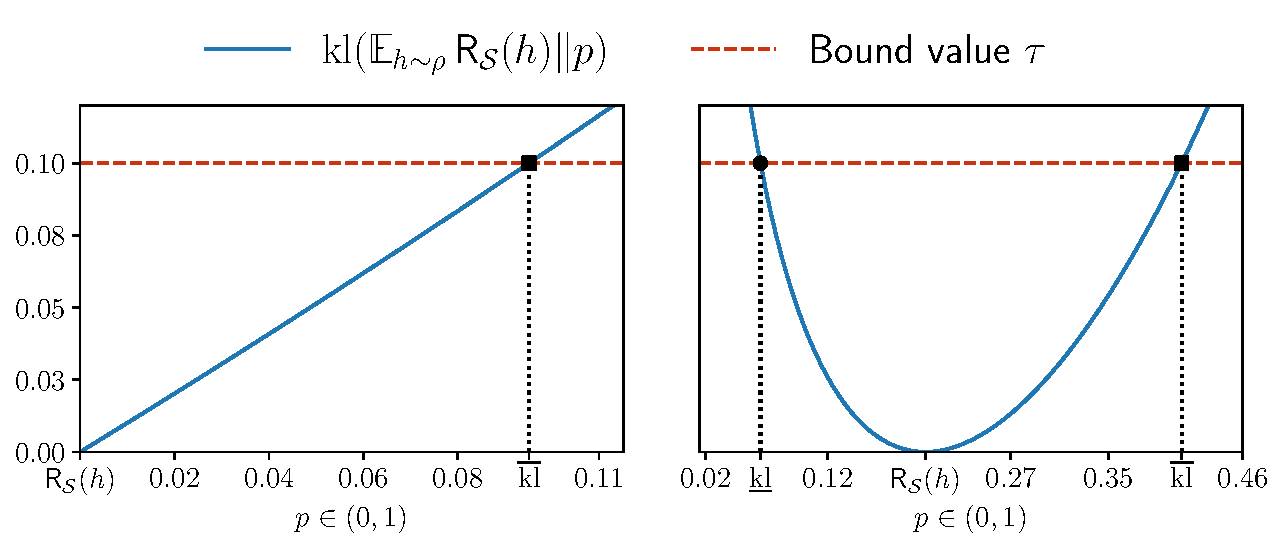
\includegraphics[width=\textwidth]{chapter_2/figures/invert_kl_optim.pdf}
    \caption[Illustration of the Functions $\klmin$ and $\klmax$]{%
    Illustration of the inverting functions of $\kl()$ for $q=\RiskLoss_{\dS}(\h)$ \st $\RiskLoss_{\dS}(\h) \in \{0.0, 0.2\}$ in two different plots.
    We plot the curve of the function $\kl(\RiskLoss_{\dS}(\h)\|\cdot)$, the bound value $\threshold=0.1$ and the two inverting functions $\klmin(\RiskLoss_{\dS}(\h)| \threshold)$ and $\klmax(\RiskLoss_{\dS}(\h)| \threshold)$ (abbreviated $\klmin$ and $\klmax$).
    The dot (\resp the square) corresponds to the solution of the minimization (\resp maximization) problem associated with $\klmin$ (\resp $\klmax$).
    }
    \label{chap:pac-bayes:fig:invert-kl-optim}
\end{figure}
Expressed as it is,  \Cref{chap:pac-bayes:eq:seeger} does not permit to upper or lower bound the expected true risk $\RiskLoss_{\D}(\h)$ contrary to \Cref{chap:pac-bayes:theorem:mcallester,chap:pac-bayes:theorem:catoni}.
In order to rewrite \Cref{chap:pac-bayes:eq:seeger} (of \Cref{chap:pac-bayes:theorem:seeger}), we define the inverting functions of $\kl()$ in the following way. 

\begin{definition}[Inverting Functions of $\kl()$] Given $\threshold\ge 0$, for any $q\in[0, 1]$, the inverting functions of the $\kl()$ are defined as
\begin{align*}
    &\klmax(q | \threshold){\defeq}\max\Big\{ p \in (0,1) \;\Big|\; \kl(q\|p) \le \threshold\Big\},\\ 
    \text{and}\quad &\klmin (q | \threshold){\defeq}\min\Big\{ p\!\in\!(0,\! 1) \;\Big|\; \kl(q\|p) \le\threshold\Big\}.
\end{align*}
\label{chap:pac-bayes:def:invert-kl}
\end{definition}

The function $\klmax()$ (\resp $\klmin()$) denotes the maximum (\resp minimum) value $p\in(0,1)$ such that the inequality $\kl(q\|p) \le \threshold$ holds.
\Cref{chap:pac-bayes:fig:invert-kl-optim} gives a graphical illustration of these inverting functions.
The values associated with the inverting functions $\klmin()$ and $\klmax()$ can be approximated and easily computed from \textsc{Pinsker}'s inequality (\Cref{ap:pac-bayes:theorem:pinsker}).
Indeed, we have
\begin{align}
    \klmax(q|\threshold) \le q + \sqrt{\frac{1}{2}\threshold} \qquad\text{and}\qquad q - \sqrt{\frac{1}{2}\threshold} \le \klmin(q|\threshold).\label{chap:pac-bayes:eq:kl-approx}
\end{align}
We present in \Cref{chap:pac-bayes:fig:invert-kl-pinsker} an illustration of the tightness of this approximation.

\begin{figure}[t]
    \centering
    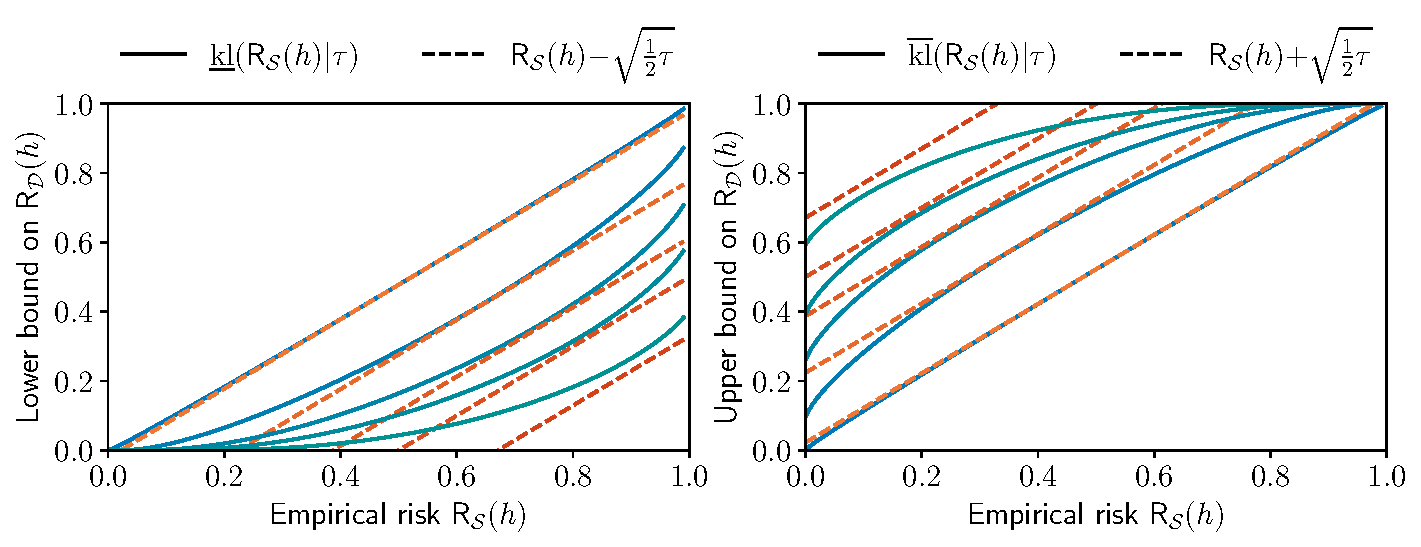
\includegraphics[width=\textwidth]{chapter_2/figures/invert_kl_pinsker.pdf}
    \caption[Illustration of the Tightness of $\klmin$ and $\klmax$]{%
    Illustration of the tightness of $\klmin()$ and $\klmax()$.
    The line represents the functions $\klmin(\cdot|\threshold)$ and $\klmax(\cdot|\threshold)$ for different values of $\threshold\in\{0.001, 0.1, 0.3, 0.5, 0.9\}$.
    On the left plot, we represent the function $\klmin(\cdot|\threshold)$ while the right plot represents the function $\klmax(\cdot|\threshold)$. 
    In the left (\resp right) plot, the lower (\resp higher) the inverting function, the smaller (\resp larger) the value of $\threshold$.
    Moreover, for each inverting function, we plot with the dotted lines its approximation through \textsc{Pinsker}'s inequality.
    }
    \label{chap:pac-bayes:fig:invert-kl-pinsker}
\end{figure}

To calculate $\klmin()$ and $\klmax()$ exactly, two optimization problems need to be solved; \citet{ReebDoerrGerwinnRakitsch2018} proposed an algorithm based on the bisection method.
We recall its pseudo-code in \Cref{chap:pac-bayes:algo:kl}. 
The principle of this algorithm is to iteratively refine the interval $[p_{\text{min}}, p_{\text{max}}]$ to which the bias $p\in(0,1]$ belongs.
When the equality $\kl(q\|p)=\threshold$ is attained or when the interval $[p_{\text{min}}, p_{\text{max}}]$ is small enough, the bias $p$ is found.

\begin{algorithm}[ht!]
   \caption{Compute $\klmax(q|\threshold)$ \resp $\klmin(q|\threshold)$ through the bisection method}
  \begin{algorithmic}
    \State{{\bf Given: } Bias $q\in[0,1]$ (the empirical risk), the bound value $\threshold\ge 0$}
    \State{{\bf Hyperparameters: } tolerance $\epsilon$, maximal number of iterations $T_\text{max}$}
    \State{$p_{\text{max}}{\leftarrow}1$ and $p_{\text{min}}{\leftarrow}q$ (resp. $p_{\text{max}}{\leftarrow}q$ and $p_{\text{min}}{\leftarrow}0$)}
    \For{$t\leftarrow 1$ to $T_{\text{max}}$}
        \State{$p = \tfrac{1}{2}\LB p_{\text{min}}{+}p_{\text{max}}\RB$}
        \State{\textbf{if} $\kl(q\|p)=\threshold$ or  $(p_{\text{min}}{-}p_{\text{max}})<\epsilon$ \textbf{ then return} $p$}
        \State{\textbf{if} $\kl(q\|p) > \threshold$ \textbf{ then } $p_\text{max}=p$ (resp. $p_\text{min}=p$)}
        \State{\textbf{if} $\kl(q\|p) < \threshold$ \textbf{ then } $p_\text{min}=p$ (resp. $p_\text{max}=p$)}
    \EndFor
     \State{\Return{$p$}}
    \end{algorithmic}
    \label{chap:pac-bayes:algo:kl}
\end{algorithm}

Moreover, \citet{ReebDoerrGerwinnRakitsch2018} found the expression of the derivatives with respect to $q$ and $\threshold$, allowing them to derive bound minimization algorithms based on gradient descent; these derivatives are defined by
\begin{align}
    \frac{\partial {\rm k(}q|\psi)}{\partial q} = \frac{\ln\frac{1-q}{1-{\rm k(}q|\psi)}-\ln\frac{q}{{\rm k(}q|\psi)}}{\frac{1-q}{1-{\rm k(}q|\psi)}-\frac{q}{{\rm k(}q|\psi)}}, \text{ and } \frac{\partial {\rm k(}q|\psi)}{\partial \psi} = \frac{1}{\frac{1-q}{1-{\rm k(}q|\psi)}-\frac{q}{{\rm k(}q|\psi)}},\label{chap:pac-bayes:eq:deriv-kl}
\end{align}
where ${\rm k}()$ is either $\klmin()$ or $\klmax()$.

Thanks to \Cref{chap:pac-bayes:def:invert-kl}, we can rewrite the bound of \Cref{chap:pac-bayes:theorem:seeger} to upper-bound the expected true risk $\EE_{\h\sim\Q}\RiskLoss_{\D}(\h)$.
With probability at least $1-\delta$ over the random choice of $\S\sim\D^\m$, we have for all $\Q\in\M(\H)$
\begin{align}
    &\EE_{\h\sim\Q}\RiskLoss_{\D}(\h) \le \klmax\LP\EE_{\h\sim\Q}\RiskLoss_{\dS}(\h) \;\middle|\; \frac{1}{\m}\!\LB\KL(\Q\|\P){+}\ln\tfrac{2\sqrt{\m}}{\delta}\RB\RP\label{chap:pac-bayes:eq:klmax-seeger}\\
    \text{and}\quad &\EE_{\h\sim\Q}\RiskLoss_{\D}(\h) \ge \klmin\LP\EE_{\h\sim\Q}\RiskLoss_{\dS}(\h) \;\middle|\; \frac{1}{\m}\!\LB\KL(\Q\|\P){+}\ln\tfrac{2\sqrt{\m}}{\delta}\RB\RP.\label{chap:pac-bayes:eq:klmin-seeger}
\end{align}

Thanks to the approximation in \Cref{chap:pac-bayes:eq:kl-approx}, one can prove that the bound of \Cref{chap:pac-bayes:theorem:seeger} is tighter than the one of \Cref{chap:pac-bayes:theorem:mcallester}.
More precisely, if we apply \Cref{chap:pac-bayes:eq:kl-approx} to \Cref{chap:pac-bayes:eq:klmax-seeger,chap:pac-bayes:eq:klmin-seeger}, we retrieve \Cref{chap:pac-bayes:eq:mcallester-1,chap:pac-bayes:eq:mcallester-2}.


\subsection{General PAC-Bayesian Bound of \citet{BeginGermainLavioletteRoy2016}}

As shown previously, the KL divergence between the posterior distribution $\Q$ and the prior distribution $\P$ is ubiquitous in PAC-Bayesian bounds.
By considering this divergence, as illustrated in \Cref{chap:pac-bayes:theorem:general-germain}, the term $\EE_{\S'\sim\D^\m}\EE_{\h'\sim\P}\exp\LB\varphi(\h', \S')\RB$ appears inevitably.
Indeed, the KL divergence $\KL(\Q\|\P)$ between $\Q$ and $\P$ can be expressed as a difference between two terms: $\EE_{\h\sim\Q}\varphi(\h,\S)$ and $\EE_{\h\sim\P}\exp\LB\varphi(\h, \S)\RB$ thanks to \citet{DonskerVaradhan1976}.
This representation is actually used to obtain a {\it change of measure inequality} which quantifies how much two expectations (coming from two densities $\Q$ and $\P$) differ.
This change of measure inequality and the expression of the KL divergence are in the following.

\begin{restatable}[\mbox{\textsc{Donsker}-\textsc{Varadhan} Variational Representation}]{proposition}{representationKL}\label{chap:pac-bayes:proposition:representation-KL}
For any hypothesis set $\H$, for any distribution $\P\in\M^{*}(\H)$ on $\H$, for any measurable function $\varphi:\H\times(\X\times\Y)^\m \rightarrow \Rbb$ \st $\EE_{\h'\sim\P}e^{\varphi(\h',\S)}<+\infty$ for all $\S\in(\X\times\Y)^\m$, we have
\begin{align*}
    \forall\S\in(\X\times\Y)^\m,\quad \forall\Q\in\M(\H),\qquad 
    &\EE_{\h\sim\Q}\varphi(\h,\S)-\ln\LP \EE_{\h\sim\P}e^{\varphi(\h,\S)}\RP \le \KL(\Q\|\P)\\
    \iff &\EE_{\h\sim\Q}\varphi(\h,\S) \le \KL(\Q\|\P)+\ln\LP \EE_{\h\sim\P}e^{\varphi(\h,\S)}\RP.
\end{align*}

When the distribution $\Q$ is defined as $\displaystyle\Q(\h)=\P(\h)\frac{e^{\varphi(\h,\S)}}{\EE_{\h'\sim\P}e^{\varphi(\h',\S)}}$, we have
\begin{align*}
    \forall\S\in(\X\times\Y)^\m,\qquad &\EE_{\h\sim\Q}\varphi(\h,\S)-\ln\LP \EE_{\h\sim\P}e^{\varphi(\h,\S)}\RP = \KL(\Q\|\P), \\
    \iff &\EE_{\h\sim\Q}\varphi(\h,\S) = \KL(\Q\|\P)+\ln\LP \EE_{\h\sim\P}e^{\varphi(\h,\S)}\RP.
\end{align*}
\end{restatable}
\begin{noaddcontents}\begin{proof}
Deferred to~\Cref{ap:pac-bayes:sec:proof-representation-KL}.
\end{proof}\end{noaddcontents}

As we can remark, this inequality resembles to the general bound of \citet{GermainLacasseLavioletteMarchand2009} (in \Cref{chap:pac-bayes:theorem:general-germain}).
Hence, the change of measure inequality appears indirectly in the PAC-Bayesian bounds making the constant term $\EE_{\S'\sim\D^\m}\EE_{\h'\sim\P}e^{\varphi(\h',\S')}$ arising in the bound.
Other divergences can be considered to obtain different constant terms (that are further upper-bounded).
For example, \citet{OhnishiHonorio2021} prove other change of measure inequalities for several divergences.
Prior to this work, \citet{BeginGermainLavioletteRoy2016} derive a new general PAC-Bayesian bound with the \textsc{Rényi} divergence defined as $\Renyi_{\lambda}(\Q\|\P) = \frac{1}{\lambda{-}1}\ln\LP\EE_{\h\sim\P}\LB\frac{\Q(\h)}{\P(\h)}\RB^\lambda\RP$ for any $\lambda> 1$.
Their bound is recalled in the following theorem.

\begin{restatable}[General PAC-Bayesian Bound of~\citet{BeginGermainLavioletteRoy2016}]{theorem}{generalbegin}\label{chap:pac-bayes:theorem:general-begin}
For any distribution $\D$ on $\X{\times}\Y$, for any hypothesis set $\H$, for any distribution $\P\in\M^{*}(\H)$ on $\H$, for any measurable function $\varphi: \H\times(\X\times\Y)^\m\to \Rbb_{*}^{+}$, for any $\lambda > 1$, for any $\delta\in(0,1]$, we have
\begin{align*}
&\PP_{\S\sim\D^{\m}}\Bigg[ \forall \Q\in\M(\H), \frac{\lambda}{\lambda{-}1}
   \ln \LB\EE_{\h{\sim}\Q}\varphi(\h,\S)\RB\\
&\hspace{3cm}\le \Renyi_{\lambda}(\Q\|\P) + \ln\LB\frac{1}{\delta}\EE_{\S'{\sim}\D^{\m}}\EE_{\h'{\sim}\P}\varphi(\h',\S')^\frac{\lambda}{\lambda{-}1}\RB \Bigg] \ge 1{-}\delta.
\end{align*}
\end{restatable}
\begin{noaddcontents}\begin{proof}
Deferred to~\Cref{ap:pac-bayes:sec:proof-general-begin}.
\end{proof}\end{noaddcontents}

Unlike \Cref{chap:pac-bayes:theorem:general-germain}, the function $(\h,\S) \mapsto \frac{\lambda}{\lambda{-}1}\ln \LB\EE_{\h{\sim}\Q}\varphi(\h,\S)\RB$ represents the generalization gap and is upper-bounded by the \textsc{Rényi} divergence $\Renyi_{\lambda}(\Q\|\P)$ and a constant term $\ln[\frac{1}{\delta}\EE_{\S'{\sim}\D^{\m}}\EE_{\h'{\sim}\P}\varphi(\h',\S')^\frac{\lambda}{\lambda{-}1}]$.
At first sight, \Cref{chap:pac-bayes:theorem:general-begin} seems very different from \Cref{chap:pac-bayes:theorem:general-germain}, however, they are actually related.
Indeed, if we replace $\varphi(\h,\S)$ by $\exp(\tfrac{\lambda{-}1}{\lambda}\varphi(\h,\S))$ and we apply \textsc{Jensen}'s inequality (\Cref{ap:tools:theorem:jensen}) on the left-hand side, we obtain with probability at least $1{-}\delta$ over the random choice of $\S{\sim}\D^\m$
\begin{align*}
    \forall \Q\in\M(\H),\quad \EE_{\h\sim\Q}\varphi(\h,\S) \le \Renyi_{\lambda}(\Q\|\P) + \ln\LB\frac{1}{\delta}\EE_{\S'{\sim}\D^{\m}}\EE_{\h'{\sim}\P}e^{\varphi(\h',\S')} \RB.
\end{align*}

This bound is slightly looser than the one of \Cref{chap:pac-bayes:theorem:general-germain}: for any $\lambda>1$ and for any distributions $\Q$ and $\P$, we have $\KL(\Q\|\P) \le \Renyi_{\lambda}(\Q\|\P)$ and $\lim_{\lambda\rightarrow 1^{+}}\Renyi_{\lambda}(\Q\|\P)=\KL(\Q\|\P)$ \citep{ErvenHarremoes2014}.
As for the general bound in \Cref{chap:pac-bayes:theorem:general-germain}, setting the function $\varphi()$ and upper-bounding the term $\EE_{\S{\sim}\D^{\m}}\EE_{\h{\sim}\P}\varphi(\h,\S)^\frac{\lambda}{\lambda{-}1}$ gives a computable bound.
Namely, \Cref{chap:pac-bayes:theorem:general-begin} allows one to obtain a \citeauthor{McAllester2003}, \citeauthor{Catoni2007} or a \citeauthor{Seeger2002}-like PAC-Bayesian bound based on the \textsc{Rényi} divergence.
For the sake of completeness, we show in \Cref{ap:pac-bayes:sec:corollary-begin} the proof of the three types of bounds based on \Cref{chap:pac-bayes:theorem:general-begin}.
Compared to \Cref{chap:pac-bayes:theorem:mcallester,chap:pac-bayes:theorem:catoni,chap:pac-bayes:theorem:seeger}, only the KL divergence is replaced by the looser \textsc{Rényi} divergence.\\

Generally speaking, all the PAC-Bayesian bounds share a common property: they bound the {\it expectation} of $\varphi()$ \wrt the posterior $\Q$.
However, it might be relevant to upper-bound $\varphi()$ for a {\it unique} hypothesis $\h\sim\Q$: this is the purpose of the {\it disintegrated} bounds.

\section{Disintegrated PAC-Bayesian Bounds}
\label{chap:pac-bayes:sec:disintegrated}

Deriving PAC-Bayesian guarantees for a unique hypothesis is tedious.
Indeed, the PAC-Bayesian theory is tailored for bounding the {\it expected} true risk.
Hence, additional derivations are needed to derive a PAC-Bayesian guarantee for a unique hypothesis.
See \citet{Langford2005,LangfordShaweTaylor2002,GermainLacasseLavioletteMarchand2009} for some examples.
To avoid this issue and to get a bound for a single hypothesis, another possible solution is to sample the hypothesis $\h\in\H$ from the posterior distribution $\AQ \in \M(\H)$.
By doing so, the gap $\LN \RiskLoss_{\D}(\h)-\RiskLoss_{\dS}(\h)\RN$ can be upper-bounded with a generalization bound.
This bound is defined in the following way.

\begin{restatable}[Disintegrated PAC-Bayesian Generalization Bound]{definition}{definitiondesintegrated}\label{chap:pac-bayes:def:disintegrated-pac-bayes}
Let $\loss: \H \times(\X{\times}\Y)\rightarrow [0,1]$ be a loss function and $\phi: [0,1]^2{\to}[0,1]$ a generalization gap. 
A {\it disintegrated} PAC-Bayesian bound is defined such that if for any distribution $\D$ on $\X\times\Y$, for any hypothesis set $\H$, for any prior distribution $\P\in\M^{*}(\H)$, for any algorithm \mbox{$A\!:\!(\X{\times}\Y)^{\m}{\times}\M^{*}(\H){\to} \M(\H)$}, there exists a function $\Phi: \M(\H){\times}\M^{*}(\H){\times}(0,1]{\to} \Rbb$ such that for any $\delta\in(0, 1]$ we have
\begin{align*}
    \PP_{\S\sim\D^\m, \h\sim\AQ}\LB \phi(\RiskLoss_{\D}(\h), \RiskLoss_{\dS}(\h)) \le \Phi\big(\AQ, \P, \delta\big) \RB \ge 1-\delta,
\end{align*}
where $\AQ \defeq A(\S, \P)$ is output by the deterministic algorithm $A$ and $\phi()$ is, for example, $\phi(\RiskLoss_{\D}(\h), \RiskLoss_{\dS}(\h)) = \LN\RiskLoss_{\D}(\h)-\RiskLoss_{\dS}(\h)\RN$.
\end{restatable}


Compared to the PAC-Bayesian bounds (see \Cref{chap:pac-bayes:def:pac-bayes}), the expectation $\EE_{\h\sim\AQ}\LB\cdot\RB$ is moved outside the indicator function: this is the disintegration.
Moreover, unlike the PAC-Bayesian bounds, the posterior $\AQ$ is obtained from an algorithm that depends on the prior $\P\in\M^{*}(\H)$ and the learning sample $\S$.
This type of bounds has been introduced in two concurrent works, \ie, \citet[Theorem~1.2.7]{Catoni2007} and \citet{BlanchardFleuret2007}.
Moreover, there exists a general disintegrated bound as for the PAC-Bayesian bounds.
We now present these three bounds by starting with the most general one.

\subsection{General Disintegrated Bound of \citet{RivasplataKuzborskijSzepesvariShaweTaylor2020}}

A general disintegrated PAC-Bayesian bound has been actually proposed very recently by \citet[Theorem~1-(i)]{RivasplataKuzborskijSzepesvariShaweTaylor2020}. 
This bound is presented below.

\begin{restatable}[General Disintegrated Bound of~\citet{RivasplataKuzborskijSzepesvariShaweTaylor2020}]{theorem}{generaldisintegratedrivasplata}\label{chap:pac-bayes:theorem:general-disintegrated-rivasplata}
For any distribution $\D$ on $\X\times\Y$, for any hypothesis set $\H$, for any prior distribution $\P\in\M^{*}(\H)$, for any measurable function $\varphi: \H\times(\X\times\Y)^\m\to \Rbb$, for any $\delta\in(0, 1]$, for any algorithm \mbox{$A\!:\!(\X{\times}\Y)^{\m}{\times}\M^{*}(\H){\to} \M(\H)$}, we have
\begin{align*}
\PP_{\S\sim\D^\m, \h\sim\AQ}\Bigg[ \varphi(\h,\S) \le \underbrace{\ln\!\LB\frac{\AQ(\h)}{\P(\h)}\RB\!+\!\ln\!\LB\frac{1}{\delta}\EE_{\S'\sim\D^\m}\EE_{\h'\sim\P}
\exp\LP\varphi(\h',\S')\RP\RB}_{\Phi(\AQ, \P, \delta)}
\Bigg] \ge 1{-}\delta,
\end{align*}
where $\AQ \defeq A(\S, \P)$ is output by the deterministic algorithm $A$.
\end{restatable}
\begin{noaddcontents}\begin{proof}
Deferred to~\Cref{ap:pac-bayes:sec:proof-general-disintegrated-rivasplata}.
\end{proof}\end{noaddcontents}

Compared to the classical PAC-Bayesian bounds, this bound holds with high probability over the random choice of the learning sample $\S\sim\D^\m$ {\it and} the hypothesis $\h\sim\AQ$.
Moreover, instead of depending on the KL divergence, the bound depends on the {\it disintegrated} KL divergence\footnote{The disintegration of the KL divergence has a slightly different meaning than the disintegration of the PAC-Bayesian bound: in the former case, the integration/expectation ``is removed'' from the divergence.} $\ln\frac{\AQ(\h)}{\P(\h)}$.
This term is the log ratio of the density of the prior $\P(\h)$ and the posterior distribution $\AQ(\h)$ for the sampled hypothesis $\h\sim\AQ$.
Intuitively, the closer the posterior density $\AQ(\h)$ to the prior density $\P(\h)$ for $\h\sim\AQ$, the lower the disintegrated KL.
As for \citet{GermainLacasseLavioletteMarchand2009}'s general bound, we need to define $\varphi()$ and upper-bound the term $\EE_{\S'\sim\D^\m}\EE_{\h'\sim\P}
\exp\LP\varphi(\h',\S')\RP$ to obtain a bound that can be computed.
Similarly to \Cref{chap:pac-bayes:theorem:general-germain,chap:pac-bayes:theorem:general-begin}, this disintegrated bound generalizes other bounds such as the one derived by \citet[Theorem~1.2.7]{Catoni2007}.

\subsection{Disintegrated Bound of \citet{Catoni2007}}

The bound of \citet[Theorem 1.2.7]{Catoni2007}, which is one of the first disintegrated bound in the literature, is recalled in the following theorem.

\begin{restatable}[Disintegrated Bound of \citet{Catoni2007}]{theorem}{disintegratedcatoni}\label{chap:pac-bayes:theorem:disintegrated-catoni}
For any distribution $\D$ on $\X\times\Y$, for any hypothesis $\H$, for any prior $\P\in\M^{*}(\H)$, for any loss $\loss: \H{\times}(\X\times\Y)^\m \to [0, 1]$, for any $\cat>0$, for any $\delta\in(0, 1]$, for any algorithm \mbox{$A\!:\!(\X{\times}\Y)^{\m}{\times}\M^{*}(\H){\to} \M(\H)$}, we have
\begin{align*}
    \PP_{\S\sim\D^\m,\h\sim\AQ}\Bigg[ \forall\Q\in\M(\H), 
    -\ln\!\LP 1{-}\LB1{-}e^{{-}\cat}\RB\EE_{\h\sim\Q}\RiskLoss_{\D}(\h)\RP&-\cat\EE_{\h\sim\Q}\RiskLoss_{\dS}(\h)\\
    &\hspace{-2cm}\le \frac{1}{\m}\LB\ln\frac{\AQ(\h)}{\P(\h)}{+}\ln\frac{1}{\delta}\RB\Bigg] \ge 1-\delta,
\end{align*}
where $\AQ \defeq A(\S, \P)$ is output by the deterministic algorithm $A$.
\end{restatable}
\begin{noaddcontents}\begin{proof}
Deferred to~\Cref{ap:pac-bayes:sec:proof-disintegrated-catoni}.
\end{proof}\end{noaddcontents}

After sampling the learning sample $\S\sim\D^\m$ and the hypothesis $\h\sim\AQ$, the obtained guarantee is similar to the one of \Cref{chap:pac-bayes:theorem:catoni}: only the KL divergence is replaced by its disintegrated counterpart.
Similar to the non-disintegrated PAC-Bayesian bound, other deviations between the true risk $\RiskLoss_{\D}(\h)$ and the empirical risk $\RiskLoss_{\dS}(\Q)$ can be considered.
For instance, \citet{BlanchardFleuret2007} proposed a bound on $\kl(\RiskLoss_{\dS}(\h)\|\RiskLoss_{\D}(\h))$. 

\subsection{Disintegrated Bound of \citet{BlanchardFleuret2007}}

The bound of \citet{BlanchardFleuret2007} is based on another proof technique called {\it Occam's hammer}.
For instance, they prove a \citet{Seeger2002}-like disintegrated PAC-Bayesian bound from this framework; it is recalled in the following theorem.

\begin{restatable}[Disintegrated Bound of \citet{BlanchardFleuret2007}]{theorem}{disintegratedblanchard}\label{chap:pac-bayes:theorem:disintegrated-blanchard}
For any distribution $\D$ on $\X\times\Y$, for any hypothesis set $\H$, for any distribution $\P\in\M^{*}(\H)$, for any loss $\loss: \H\times(\X\times\Y)\to \{0,1\}$, for any $\blan>1$, for any $\delta\in(0, 1]$, for any algorithm \mbox{$A\!:\!(\X{\times}\Y)^{\m}{\times}\M^{*}(\H){\to} \M(\H)$}, we have
\begin{align*}
\PP_{\S\sim\D^\m, \h\sim\AQ}\LB \kl_{+}(\RiskLoss_{\dS}(\h)\|\RiskLoss_{\D}(\h)) \le  \frac{1}{\m}\LB\ln\frac{\blan+1}{\delta}+\LP1+\frac{1}{\blan}\RP\ln_{+}\frac{\AQ(\h)}{\P(\h)}\RB \RB \ge 1-\delta,
\end{align*}
where $\AQ \defeq A(\S, \P)$ is output by the deterministic algorithm $A$, the $\ln_{+}(x)=\max(\ln(x), 0)$ and $\kl_{+}(\RiskLoss_{\dS}(\h)\|\RiskLoss_{\D}(\h))=\kl(\RiskLoss_{\dS}(\h)\|\RiskLoss_{\D}(\h))$ if $\RiskLoss_{\dS}(\h)<\RiskLoss_{\D}(\h)$ and 0 otherwise.
\end{restatable}
\begin{noaddcontents}\begin{proof}
Deferred to~\Cref{ap:pac-bayes:sec:proof-disintegrated-blanchard}.
\end{proof}\end{noaddcontents}

Similarly to \citet{Catoni2007}, this bound is parametrized: the tightness depends on the parameter $\blan>1$.
However, the optimal parameter depends on the log ratio $\ln_{+}\frac{\AQ(\h)}{\P(\h)}$ and cannot be set in advance since we don't know the sampled $\S\sim\D^\m$.

\section{Conclusion and Summary}

This chapter introduces generalization bounds from the PAC-Bayesian literature.
These bounds allow deriving theoretical guarantees for some machine learning models, \eg, the majority vote.
They are further useful to derive practical learning algorithms guaranteeing that the model is not too sensitive to overfitting; see \Cref{part:contrib-pac-bayes}.
Indeed, in \Cref{chap:mv-robustness}, we derive a new self-bounding learning algorithm that minimizes a PAC-Bayesian generalization bound for the adversarially robust setting.
Roughly speaking, we derive surrogates similar to \Cref{chap:pac-bayes:eq:2gibbs} to obtain guarantees and derive learning algorithms that ``robustify'' the majority vote.
Then, \Cref{chap:mv} introduces our contributions to minimizing of the PAC-Bayesian C-Bound, which aims to minimize the true risk of the majority vote.
Lastly in \Cref{part:contrib-pac-bayes}, we introduce the stochastic majority vote (where the distribution $\Q$ follows a Dirichlet distribution) in \Cref{chap:mv-sto}. 
This majority vote allows using easily a PAC-Bayesian bound on the expected true risk to learn such a classifier.\\

However, the main drawback of the PAC-Bayesian generalization bounds is that we bound $\EE_{\h\sim\Q}\varphi(h,\S)$ instead of $\varphi(h,\S)$.
In contrast, the disintegrated bounds allow us to bound the term $\varphi(h,\S)$, which makes more sense if we want to deal with a unique hypothesis $h\sim\Q$.
\Cref{part:contrib-disintegrated} shows the potential of such bounds for the analysis of the generalization of over-parametrized models.
Indeed, \Cref{chap:dis-pra} shows the first application of such bounds in practice, notably with over-parametrized models; this also leads to the derivation of new disintegrated bounds that are more appealing to optimization.
Lastly, \Cref{chap:dis-mu} introduces new perspectives based on these bounds since we can derive generalization bounds that do not depend on classical complexity measures such as the VC-Dimension or the Rademacher complexity (see \Cref{chap:intro:sec:bound}).